% =====================================================================================
% Chapter 5 - concise version (v3: caching, batch, SHAP, database and latency details restored)
% Required packages in the preamble: graphicx, booktabs, amsmath.
% Figures: copy the folder Demo/docs/figures into the thesis project as figures/.
% \tbd marks values to be filled in after the benchmark is run with all seven checkpoints.
% =====================================================================================
\providecommand{\tbd}{\underline{\hspace{1.2cm}}}

\chapter{SYSTEM DESIGN AND IMPLEMENTATION}
\label{chap:system_design}

This chapter describes how the TriMVPP framework presented in Chapter~4 is implemented as an interactive web-based system. It covers the system architecture, the integration of foundation models and bioinformatics resources, the single-variant and batch workflows, data management and deployment, the web interface, and the system's response time.

% -------------------------------------------------------------------------------------
\section{System Architecture}
\label{sec:system_architecture}

The system follows a three-tier client--server architecture (Fig.~\ref{fig:system_architecture}) that separates user interaction, AI processing, and data management, so that heavy annotation and inference tasks do not block the user interface. The React frontend communicates with a FastAPI backend through REST for single-variant queries and Server-Sent Events (SSE) for streaming batch results. The backend manages the complete inference workflow and runs long operations, such as VEP annotation and GPU computation, in background threads. All data resources, including the PostgreSQL database and the bioinformatics references, are deployed locally, which keeps annotation results consistent and means that the system does not depend on external web services.

The presentation tier is a single-page application that keeps its state in the browser: the selected variant and feature configuration are stored in the URL so that a result can be shared or reopened, and batch progress is kept in session storage so that it is not lost when the user changes pages. The application tier checks the format of every request and response and gives each request an ID, which is used for logging and for measuring the time of each stage. The data tier combines a relational database, which stores variants, features, and predictions, with read-only reference resources: the GRCh38 genome and Ensembl proteome, the SpliceAI archive, and two FAISS indexes, each containing $23{,}208$ reference embeddings of one foundation model.

\begin{figure}[htbp]
    \centering
    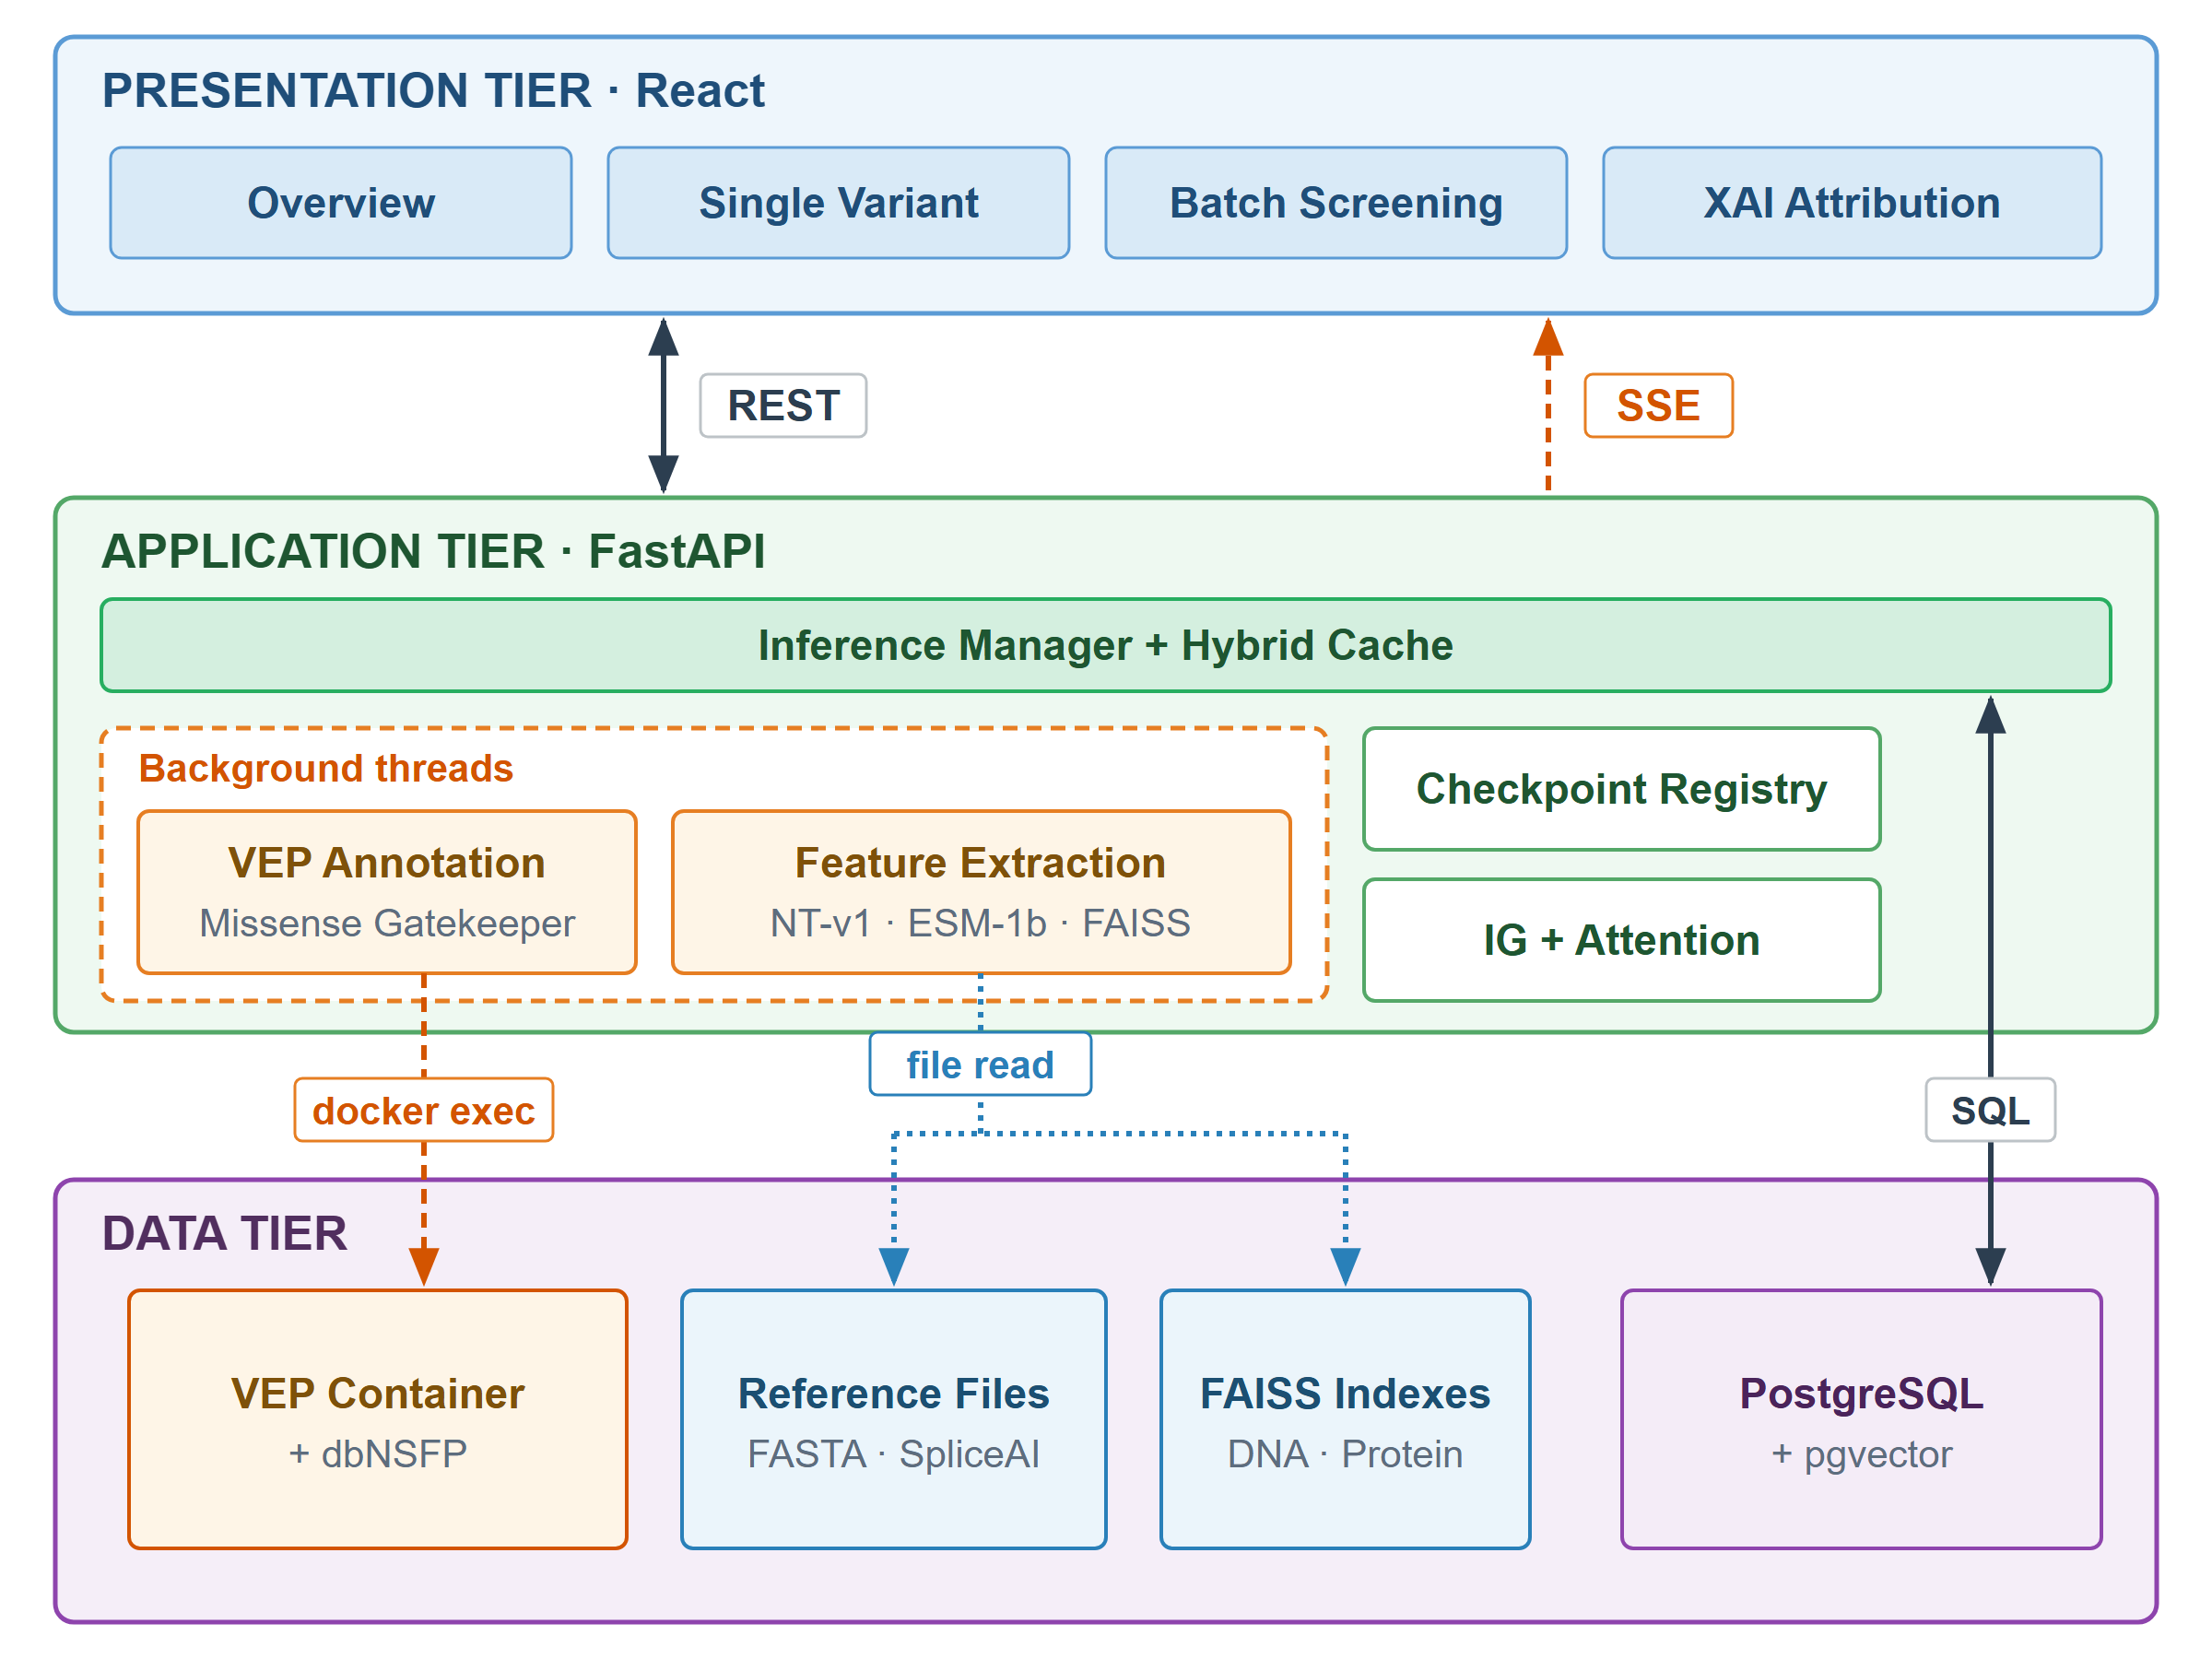
\includegraphics[width=0.95\textwidth]{figures/5.1.png}
    \caption{Three-tier architecture of the TriMVPP system.}
    \label{fig:system_architecture}
\end{figure}

% -------------------------------------------------------------------------------------
\section{Artificial Intelligence Model and Bioinformatics Integration}
\label{sec:ai_integration}

\subsection{Feature Extraction Pipeline}

To avoid a long delay on the first request, the backend loads the foundation models, sequence and FAISS indexes, and normalization files once at startup and performs a warm-up forward pass before accepting requests. Each variant, specified as \texttt{chr:pos:ref>alt} on GRCh38, is annotated by the offline Ensembl VEP service, which selects the MANE Select or canonical transcript and provides the consequence, the protein position, and the eleven core biological features: two population allele frequencies from the VEP cache and nine conservation scores from dbNSFP. AlphaMissense, REVEL, and ClinVar annotations are collected at the same time for comparison.

Since TriMVPP is trained only on missense single-nucleotide variants, a missense gatekeeper rejects all other consequence types, and the reference allele and amino acid are checked against the local GRCh38 genome and proteome to detect inputs from a wrong genome build. For accepted variants, the nine SpliceAI features are read from the compressed SpliceAI archive through a custom tabix reader that decompresses only the blocks surrounding the variant. The DNA and protein windows ($1{,}001$~bp and $501$~aa) centered on the mutation are encoded by NT-v1 500M\footnote{\url{https://huggingface.co/InstaDeepAI/nucleotide-transformer-500m-human-ref}} and ESM-1b 650M\footnote{\url{https://huggingface.co/facebook/esm1b_t33_650M_UR50S}} in FP32 precision, and the resulting embeddings are used to compute the geometric descriptors. For each foundation model, four descriptors are calculated: the Euclidean and cosine distances between the reference and alternative embeddings, the Euclidean distance relative to the norm of the reference embedding, and the local intrinsic dimensionality estimated from $k = 64$ nearest neighbors in the corresponding FAISS index. Table~\ref{tab:tabular_features} lists the resulting $28$ tabular features, which are standardized with the imputers and scalers fitted on the training set.

\begin{table}[htbp]
    \centering
    \caption{Tabular features extracted for each variant.}
    \label{tab:tabular_features}
    \begin{tabular}{lp{0.54\textwidth}c}
        \toprule
        \textbf{Group} & \textbf{Features} & \textbf{Count} \\
        \midrule
        Allele frequency & 1000 Genomes and gnomAD exomes & 2 \\
        Conservation & Three phyloP, three phastCons, and three GERP-based scores & 9 \\
        SpliceAI & Four delta scores, four delta positions, and the maximum delta score & 9 \\
        Geometry & Four descriptors for each of the DNA and protein embeddings & 8 \\
        \midrule
        Total & & 28 \\
        \bottomrule
    \end{tabular}
\end{table}

\subsection{Ablation-Aware Model Routing}

The web interface provides three feature groups, each controlled by a single switch: \textit{DNA}, \textit{Protein}, and \textit{Bio + Geom + SpliceAI}. Since disabling all groups is not allowed, the system supports seven configurations (Table~\ref{tab:ablation_configs}). A checkpoint registry links each configuration to its trained checkpoint and determines the architecture directly from the stored weights, so that new checkpoints can be added without changing the code. The full configuration uses the \texttt{RouterExpertCorrection} model ($6{,}462{,}728$ parameters, router temperature $T = 0.3074$, learnable correction weight $\beta$), while the six reduced configurations use \texttt{MultiStrategyFusionModel} checkpoints. Each checkpoint uses its own MCC-optimal threshold $\tau$ (e.g., $\tau = 0.6376$ for the full configuration), and a variant is classified as \textit{Pathogenic} if $p \geq \tau$ and as \textit{Benign} otherwise. A default of $\tau = 0.5$ is used only when no calibrated threshold is available. The biological, geometric, and SpliceAI features share one switch, so that they are always enabled or disabled together.

\begin{table}[htbp]
    \centering
    \caption{Feature-ablation configurations supported by the checkpoint registry.}
    \label{tab:ablation_configs}
    \begin{tabular}{clcc}
        \toprule
        \textbf{Key} & \textbf{Active feature groups} & \textbf{Architecture} & \textbf{SHAP players} \\
        \midrule
        \texttt{111} & DNA, Protein, Bio + Geom + SpliceAI & RouterExpertCorrection & 30 \\
        \texttt{110} & DNA, Protein & MultiStrategyFusion & 2 \\
        \texttt{101} & DNA, Bio + Geom + SpliceAI & MultiStrategyFusion & 29 \\
        \texttt{011} & Protein, Bio + Geom + SpliceAI & MultiStrategyFusion & 29 \\
        \texttt{100} & DNA & MultiStrategyFusion & 1 \\
        \texttt{010} & Protein & MultiStrategyFusion & 1 \\
        \texttt{001} & Bio + Geom + SpliceAI & MultiStrategyFusion & 28 \\
        \bottomrule
    \end{tabular}
\end{table}

\subsection{Integrated Explainability}

Instead of using an external explainability library, the inference engine includes its own GPU-based permutation Shapley estimator. Each active embedding displacement ($\boldsymbol{\delta}_{\text{DNA}}$ or $\boldsymbol{\delta}_{\text{Prot}}$) is treated as one player and each of the $28$ standardized tabular features as a separate player, giving $n = 30$ players for the full configuration. A missing player is replaced by a zero baseline, that is, a zero displacement vector or a zero standardized feature value. The engine generates $64$ random permutations together with their reversed orders, which makes the estimate more stable, and for each of the resulting $128$ permutations adds the players one by one. The attribution (contribution) of a player is the average change in the model logit when that player is added. All $128 \times (n + 1)$ feature combinations, $3{,}968$ for the full configuration, are evaluated on the GPU in large batches rather than one at a time. Because the changes along each permutation add up to the total change in the logit, the attributions satisfy the efficiency property, apart from small rounding errors:
\[
    \sum_{i=1}^{n} \phi_i = f(\mathbf{x}) - f(\mathbf{0}).
\]
Because the attributions are computed in the same request, every prediction comes with its feature-level explanation. Treating each embedding displacement as a single player keeps the explanation easy to read: it shows how much each sequence type contributes as a whole, while the biological, splicing, and geometric features are shown one by one.

% -------------------------------------------------------------------------------------
\section{Data Flow and Communication Protocols}
\label{sec:data_flow}

\subsection{Single-Variant Inference with Hybrid Lazy-Caching}

To keep the system fast for interactive use, extracted features and predictions are cached separately, so that each request follows one of the three paths in Fig.~\ref{fig:single_sequence}.

\begin{itemize}
    \item \textit{Cache hit:} a valid prediction exists for the variant and the selected configuration, and it is returned directly from the database.
    \item \textit{Feature reuse:} valid features exist, but the prediction must be recomputed because the user changed the feature configuration, enabled \textit{Live Bypass}, or the checkpoint was updated. The stored embeddings and unscaled features are reloaded, and only normalization, classification, and explanation are executed again.
    \item \textit{Cache miss:} no valid features exist, and the full pipeline is executed.
\end{itemize}

On a cache miss, VEP annotation is slow but does not use the GPU. It is therefore started in a background thread while the DNA window is extracted, the SpliceAI scores are read, and NT-v1 encodes the DNA sequences, since none of these steps depends on the VEP result. Protein extraction has to wait, because the protein isoform and residue position are provided by VEP and must first pass the missense gatekeeper. The extracted features are saved before classification, so that the slow extraction does not need to be repeated if a later step fails.

Cached results are given a version to avoid using outdated data. Features are stored with a hash of the extraction settings, such as the foundation model names, window lengths, compute device, and numerical precision, while predictions also store the name and modification time of the checkpoint that produced them. Therefore, when one of these settings or the model changes, the affected cached results are no longer used.

\begin{figure}[htbp]
    \centering
    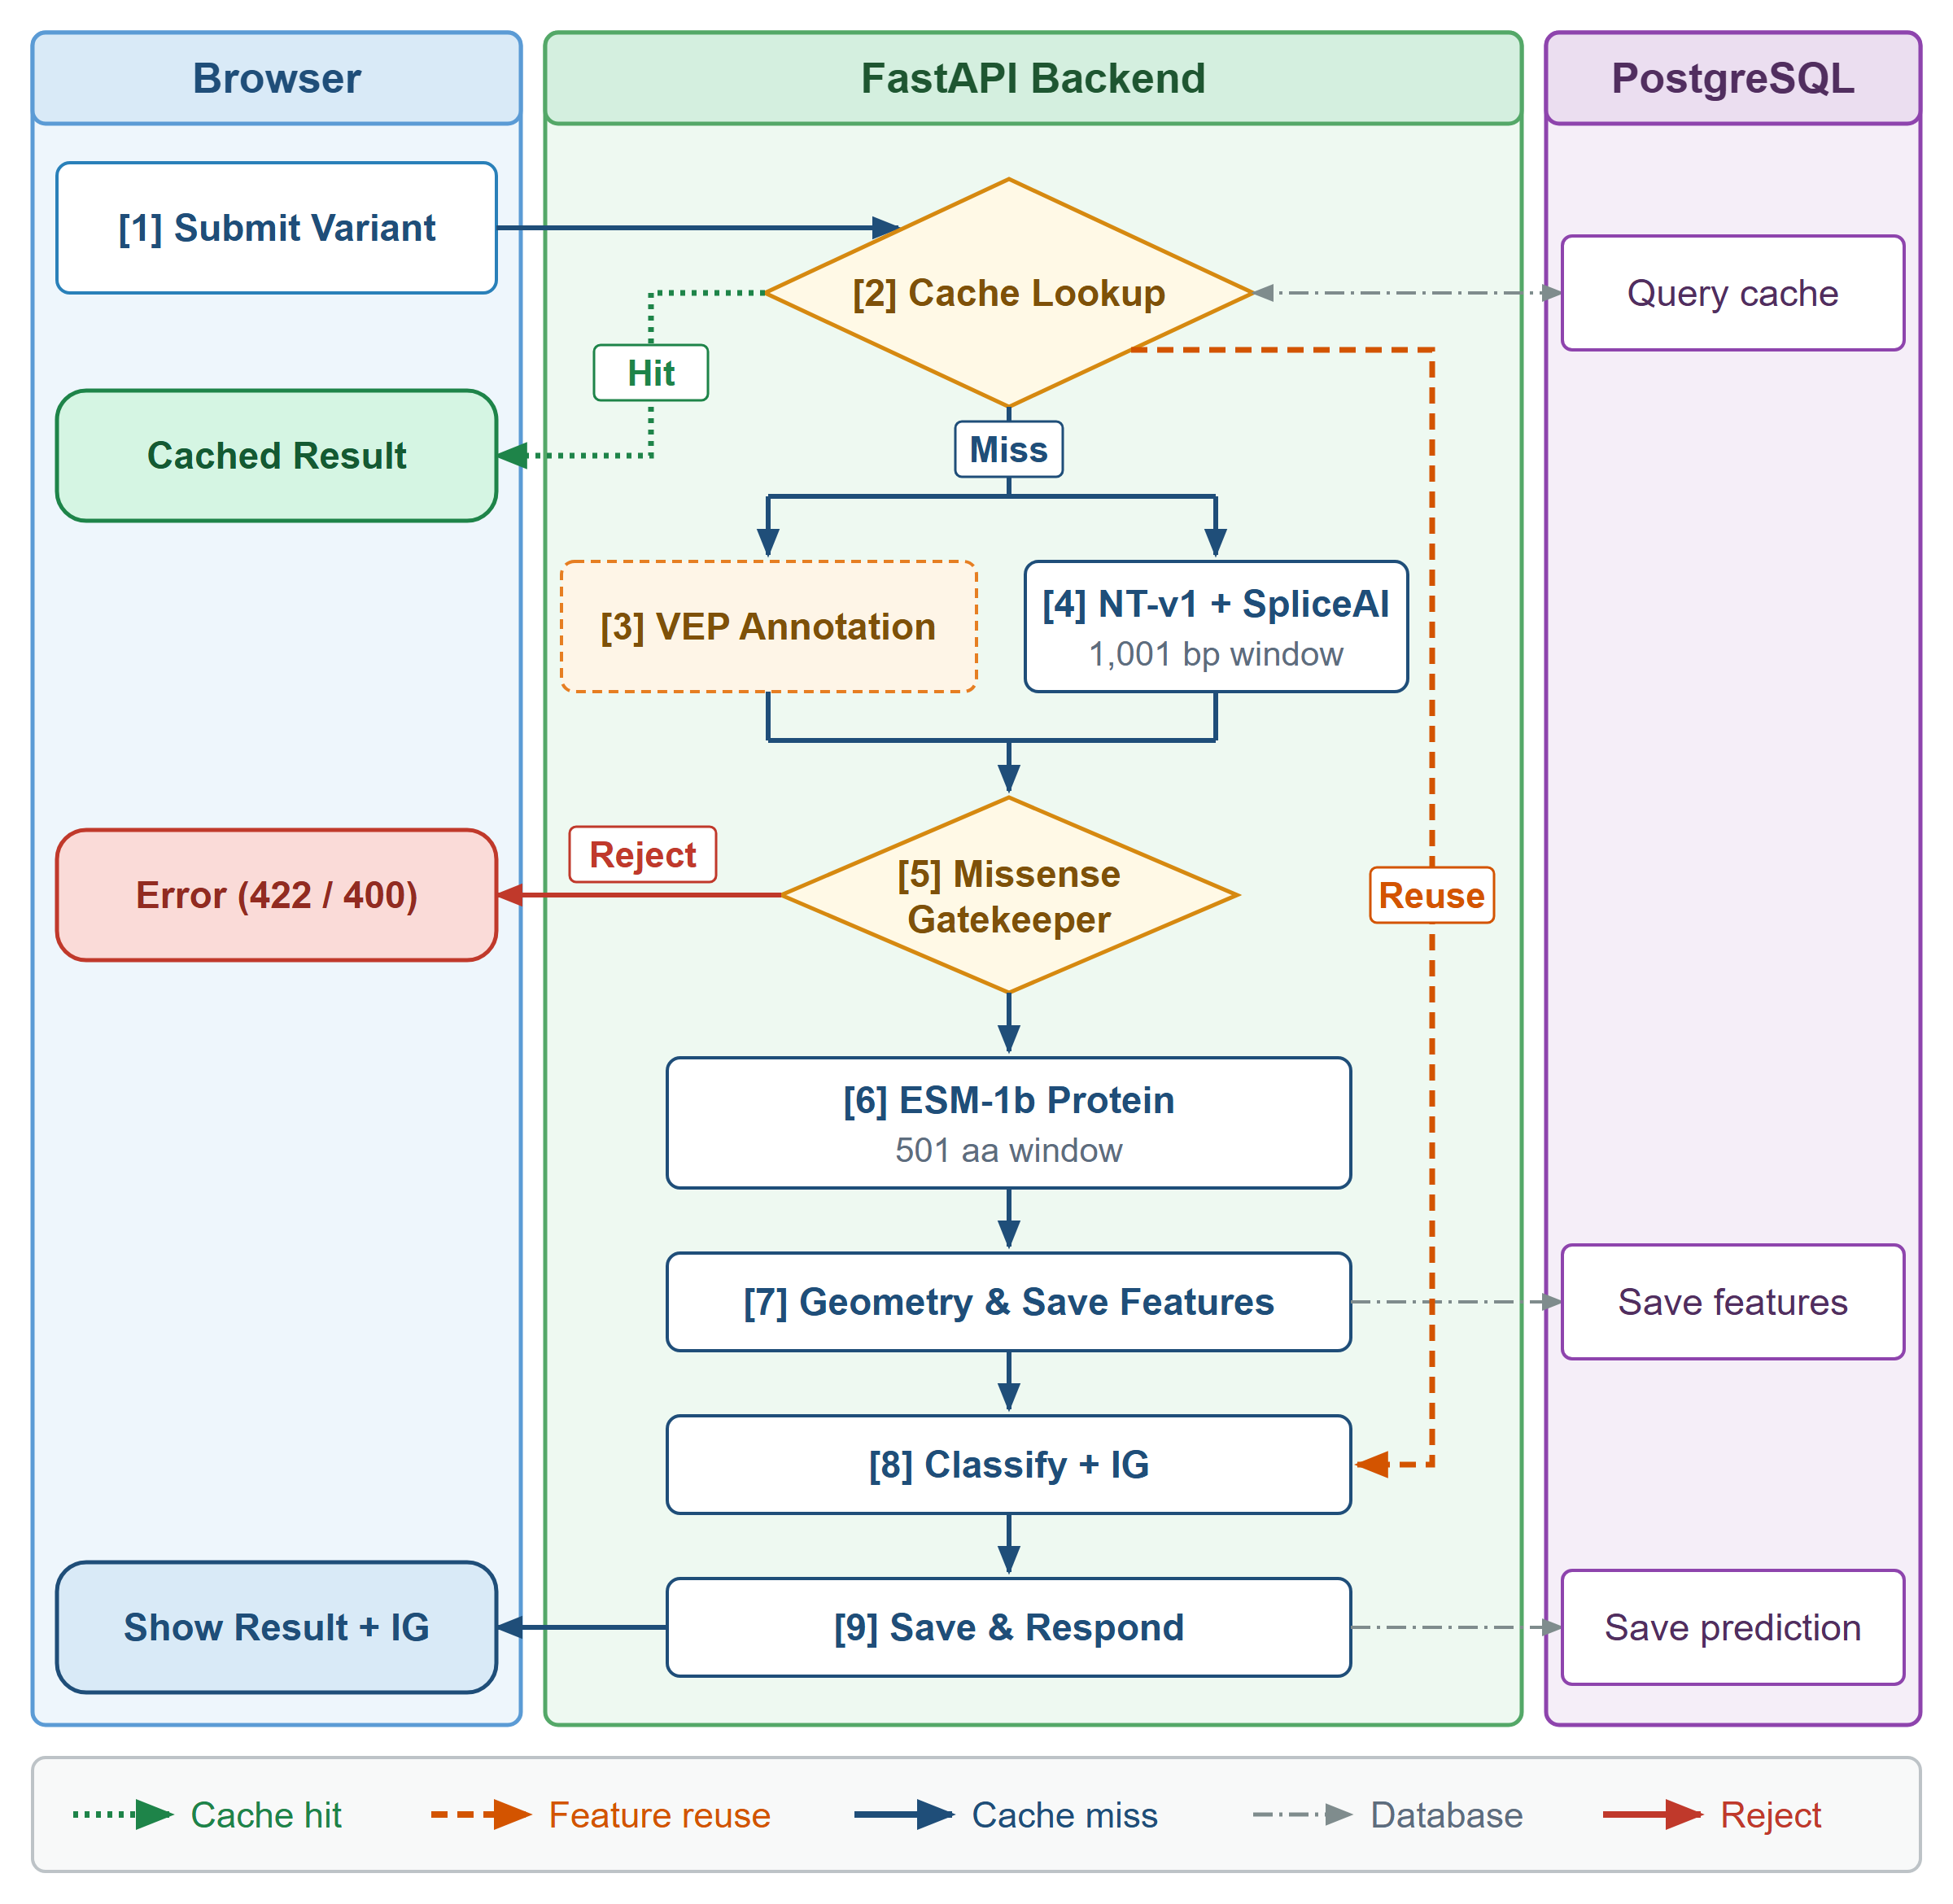
\includegraphics[width=0.95\textwidth]{figures/5.2.png}
    \caption{Single-variant inference workflow with hybrid lazy-caching.}
    \label{fig:single_sequence}
\end{figure}

\subsection{Batch Screening via Server-Sent Events}

Batch screening (Fig.~\ref{fig:batch_sse}) accepts a variant file (VCF, CSV, TXT, Parquet, or Excel) or a built-in $10$-variant benchmark cohort and streams results through SSE, which avoids HTTP timeouts and shows progress in real time. Uploaded files are read with automatic detection of common column names, and duplicate variants are removed. Processing then follows three stages:

\begin{enumerate}
    \item \textit{Cohort annotation:} all uncached variants are annotated in a single VEP run, which uses several processes for cohorts of more than $50$ variants, and SpliceAI scores are read for the accepted variants.
    \item \textit{Micro-batched feature extraction:} accepted variants are encoded in micro-batches of up to eight variants per foundation model forward pass. A micro-batch that exceeds the available GPU memory is automatically split in half and run again.
    \item \textit{Classification and streaming:} each variant is classified and explained individually, and its result is sent as soon as it is ready, so the result table in the browser is updated step by step instead of waiting for the whole cohort.
\end{enumerate}

The stream uses four event types: a classified variant, a variant skipped by the gatekeeper or coordinate validation, completion of the cohort with final statistics, and a system-level error. A single invalid variant is therefore reported with the reason, and the rest of the cohort continues to run.

\begin{figure}[htbp]
    \centering
    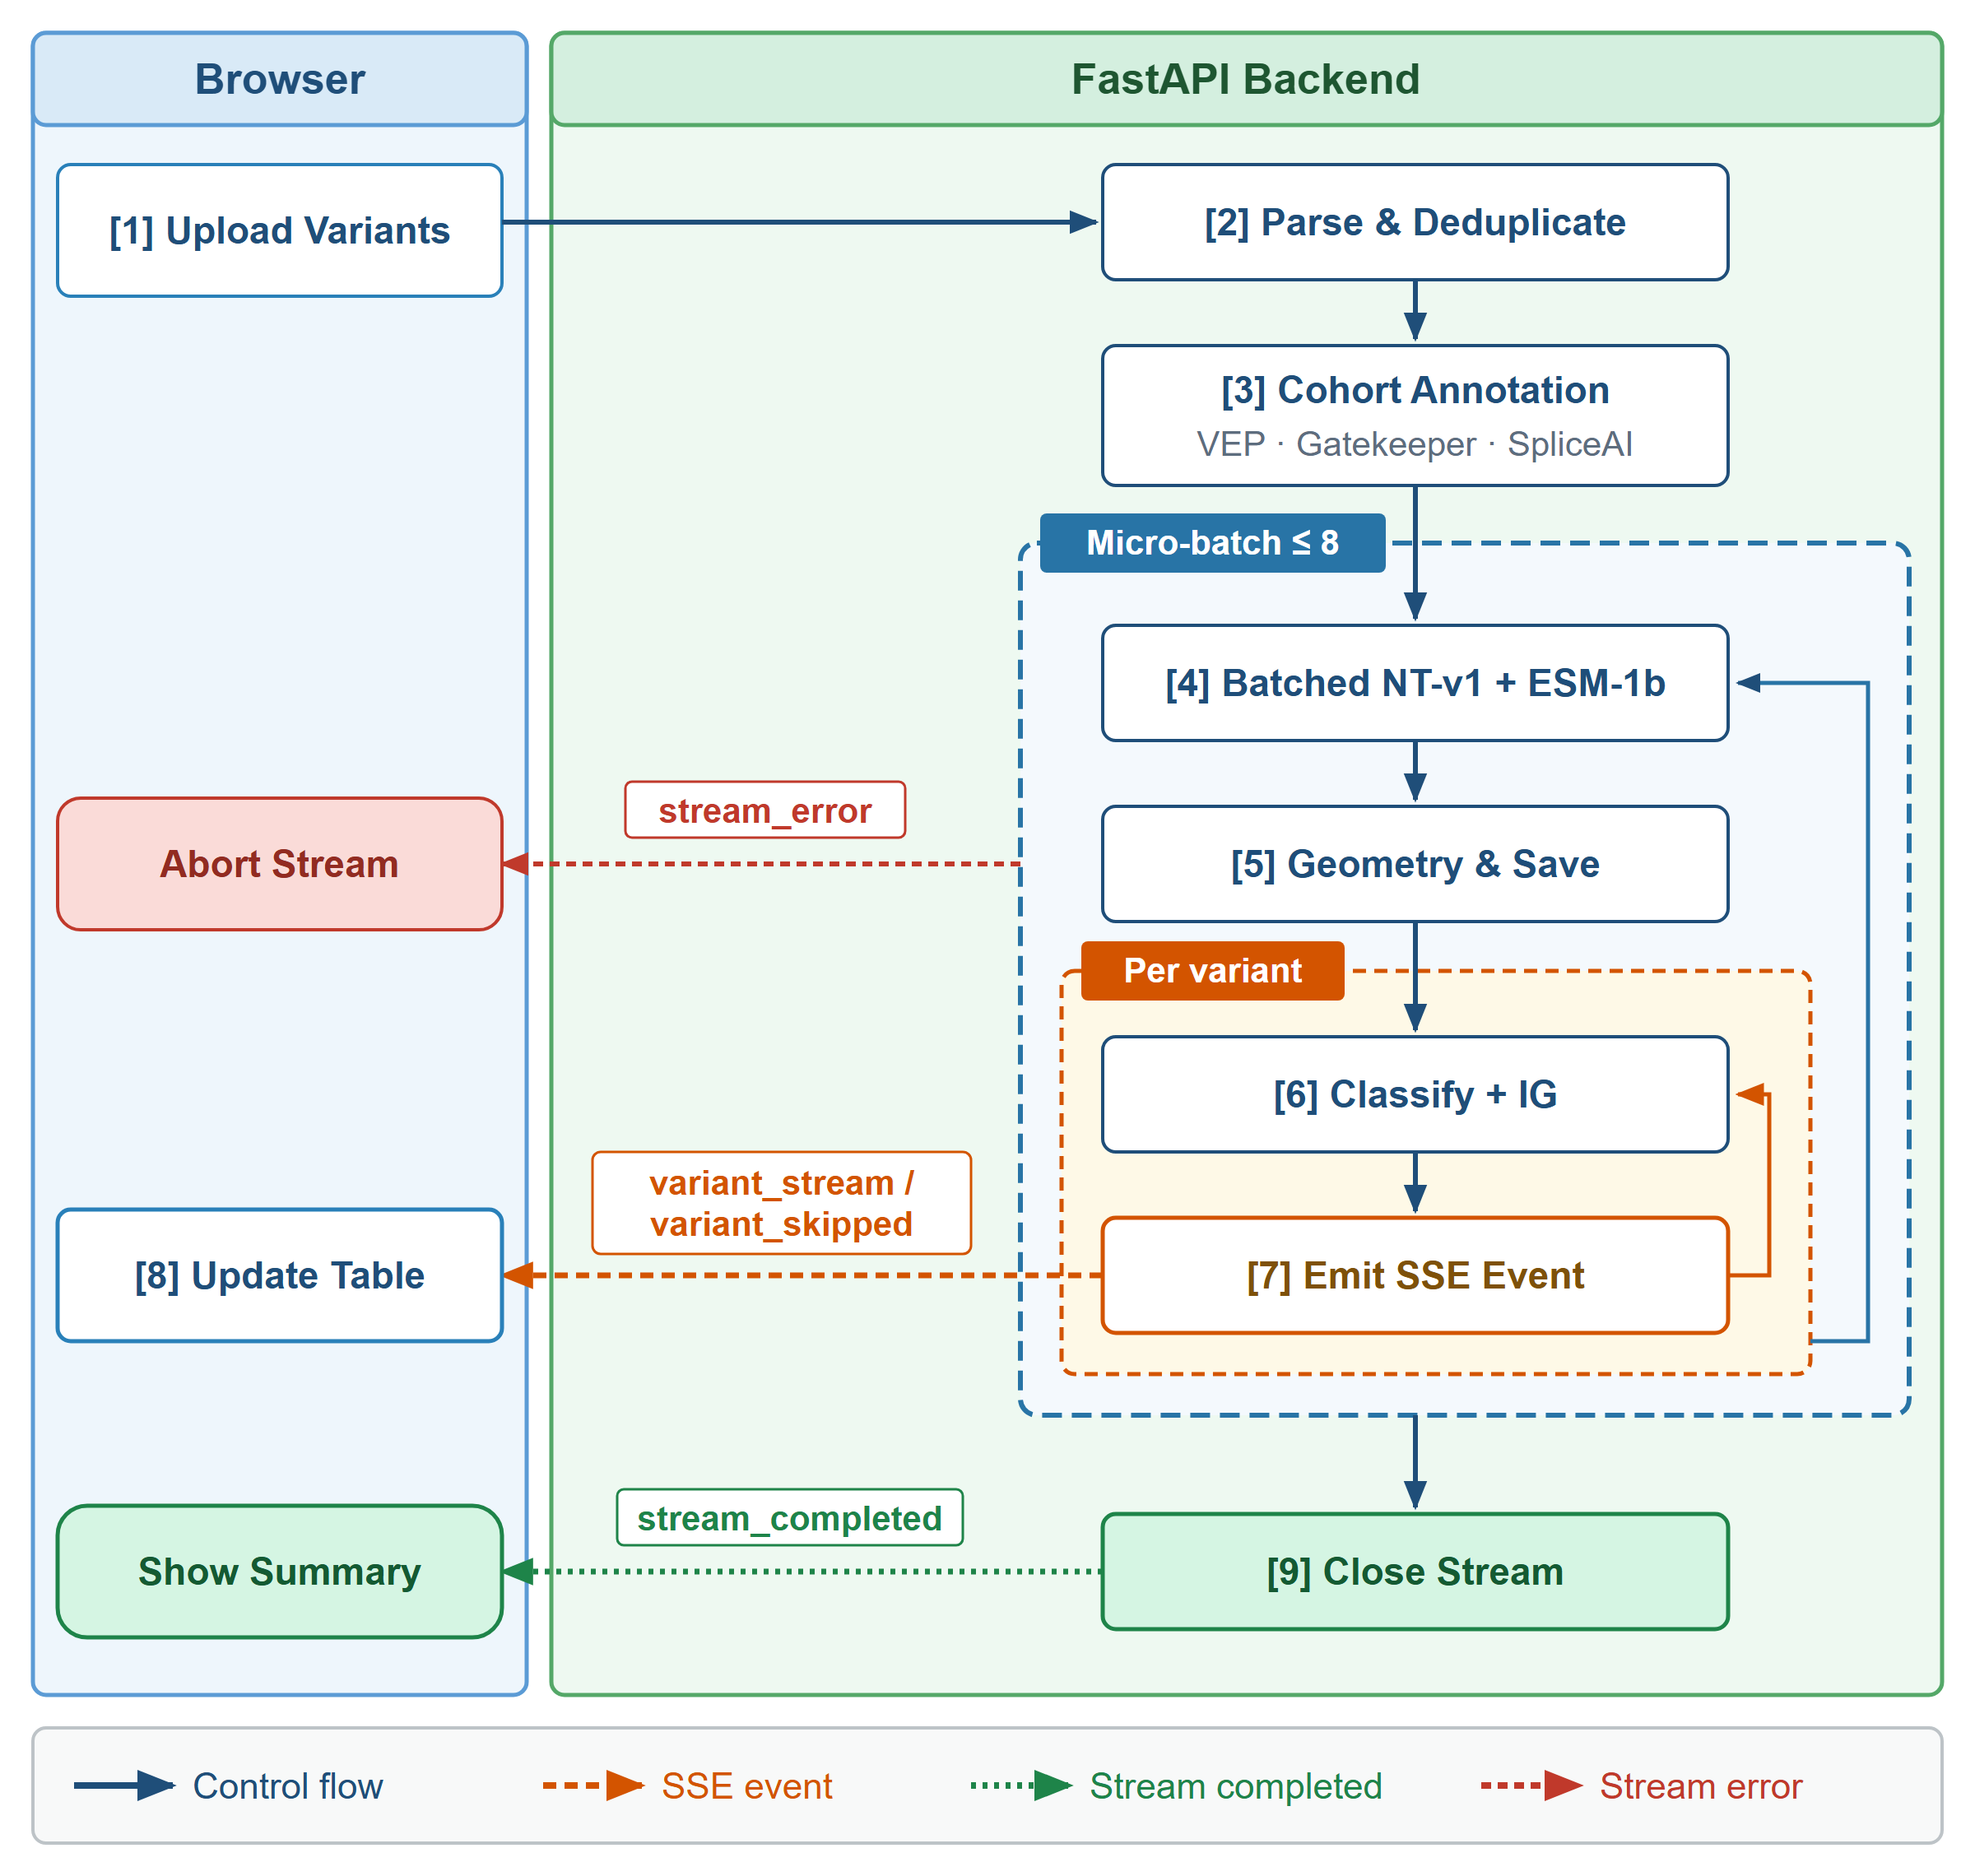
\includegraphics[width=0.95\textwidth]{figures/5.3.png}
    \caption{Batch screening workflow with micro-batched inference and SSE streaming.}
    \label{fig:batch_sse}
\end{figure}

% -------------------------------------------------------------------------------------
\section{Data Management and Deployment}
\label{sec:db_deployment}

The PostgreSQL database consists of three tables linked by foreign keys with cascading deletion (Table~\ref{tab:db_schema}). Separating features from predictions follows the caching strategy in Section~\ref{sec:data_flow}: one feature record is used for all seven configurations of a variant, and a unique index on the variant and configuration keeps at most one active prediction for each of them.

\begin{table}[htbp]
    \centering
    \caption{Main tables of the PostgreSQL database.}
    \label{tab:db_schema}
    \begin{tabular}{lp{0.22\textwidth}p{0.38\textwidth}}
        \toprule
        \textbf{Table} & \textbf{Number of records} & \textbf{Main contents} \\
        \midrule
        \texttt{variants} & One record per GRCh38 variant & Gene, consequence, protein change, and normalized ClinVar label \\
        \addlinespace
        \texttt{inference\_features} & One record per variant & Four $1{,}280$-dimensional embeddings, unscaled tabular features, VEP annotation, and hash of the extraction settings \\
        \addlinespace
        \texttt{predictions} & Up to seven records per variant & Probability, label, AlphaMissense and REVEL scores, Shapley attributions, and model version \\
        \bottomrule
    \end{tabular}
\end{table}

The reference and alternative embeddings are stored as \texttt{pgvector} columns and are rounded to FP16 precision before storage to match the format used during training. The database only saves and loads these vectors, while nearest-neighbor search is performed by the FAISS indexes in memory. Tabular features are stored unscaled, so that normalization can be repeated without running the extraction again. All writes use the insert-or-update (upsert) operation of PostgreSQL, so requests that are repeated or sent at the same time update the existing record instead of creating duplicates.

The system uses a hybrid deployment: PostgreSQL and the offline VEP service run in Docker containers, which keeps their dependencies separate, while the FastAPI backend runs directly on the host machine to access the GPU through CUDA and loads the foundation models on the GPU only once at startup. The backend calls the VEP container locally, with the reference genome, VEP cache, and dbNSFP database mounted from the host, so no variant data are sent outside the workstation. A single startup script starts the database, backend, and frontend, while the VEP container is set up separately and must be running before annotation requests are sent. The main technologies are summarized in Table~\ref{tab:tech_stack}.

\begin{table}[htbp]
    \centering
    \caption{Technology stack of the TriMVPP system.}
    \label{tab:tech_stack}
    \begin{tabular}{ll}
        \toprule
        \textbf{Layer} & \textbf{Technologies} \\
        \midrule
        Frontend & React 19, TypeScript, Vite, Tailwind CSS, Recharts \\
        Backend & Python 3.10, FastAPI, Uvicorn, Pydantic, SQLAlchemy \\
        Deep learning & PyTorch 2.4 (CUDA 12.1), Hugging Face Transformers, FAISS \\
        Database & PostgreSQL 16 with \texttt{pgvector} (Docker) \\
        Bioinformatics & Ensembl VEP 116 with dbNSFP 5.3.1a (Docker), SpliceAI MANE v1.4, pyfaidx \\
        \bottomrule
    \end{tabular}
\end{table}

% -------------------------------------------------------------------------------------
\section{Web Interface}
\label{sec:web_interface}

The web interface (Fig.~\ref{fig:web_interface}) provides four views. The overview page (a) introduces the system and links to each module. The single-variant view (b) accepts a GRCh38 coordinate and the three feature switches, and displays the predicted probability and label together with ClinVar, AlphaMissense, and REVEL; a \textit{Live Bypass} option makes the system compute the prediction again. The batch view (c) shows the streaming progress, the numbers of accepted and rejected variants, and a live table of the variants that are most likely to be pathogenic. The explainability view (d) presents the Shapley attributions of a selected variant as a bar chart with positive and negative contributions. When a result is opened in another view, its variant and feature configuration are kept.

\begin{figure}[htbp]
    \centering
    % Replace each box with \includegraphics[width=\linewidth]{figures/5.4x.png}
    \begin{minipage}{0.48\textwidth}\centering
        \fbox{\parbox{0.95\linewidth}{\centering\vspace{1.6cm}\textit{[Overview page]}\vspace{1.6cm}}}\\[2pt]
        \small (a) System overview
    \end{minipage}\hfill
    \begin{minipage}{0.48\textwidth}\centering
        \fbox{\parbox{0.95\linewidth}{\centering\vspace{1.6cm}\textit{[Single-variant view]}\vspace{1.6cm}}}\\[2pt]
        \small (b) Single-variant inspection
    \end{minipage}\\[8pt]
    \begin{minipage}{0.48\textwidth}\centering
        \fbox{\parbox{0.95\linewidth}{\centering\vspace{1.6cm}\textit{[Batch view]}\vspace{1.6cm}}}\\[2pt]
        \small (c) Batch screening
    \end{minipage}\hfill
    \begin{minipage}{0.48\textwidth}\centering
        \fbox{\parbox{0.95\linewidth}{\centering\vspace{1.6cm}\textit{[Explainability view]}\vspace{1.6cm}}}\\[2pt]
        \small (d) Explainability analysis
    \end{minipage}
    \caption{Main views of the TriMVPP web interface.}
    \label{fig:web_interface}
\end{figure}

% -------------------------------------------------------------------------------------
\section{Latency Evaluation}
\label{sec:latency}

Latency was measured on a workstation with an AMD Ryzen~7 8745H CPU, 32~GB of RAM, and an NVIDIA GeForce RTX 4060 Laptop GPU (8~GB VRAM) running Windows~11, with all inference in FP32. Loading the models at startup takes approximately \tbd{}~s and \tbd{}~GB of GPU memory and is excluded from the measurements. % TODO: fill in after the FP32 benchmark
Latency was recorded by the backend, from the time a request is received until the response is created, with one user sending requests one after another on the $10$-variant benchmark cohort (Table~\ref{tab:latency_benchmarks}). For batch screening, the total is the time until the stream completes. The reported values therefore do not include JSON conversion, network transfer, and browser display time, and they apply only to this hardware configuration.

% TODO: fill in the latency column once all seven checkpoints are available.
\begin{table}[htbp]
    \centering
    \caption{Server-side processing latency across execution paths on the reference workstation.}
    \label{tab:latency_benchmarks}
    \begin{tabular}{llr}
        \toprule
        \textbf{Scenario} & \textbf{Execution path} & \textbf{Latency} \\
        \midrule
        Single new variant & Full cache miss & \tbd{} s / variant \\
        Batch cohort ($10$ variants) & Full cache miss & \tbd{} s total \\
        Configuration change / Live Bypass & Feature reuse & \tbd{} s / query \\
        Repeated query & Full cache hit & \tbd{} ms / query \\
        \bottomrule
    \end{tabular}
\end{table}

Batch processing reduces the average cost to \tbd{}~s per variant, which is \tbd{}$\times$ faster than sending single-variant requests one by one, mainly because VEP is run once for the whole cohort and the foundation models process several variants per forward pass. Once a variant's features are stored, changing the feature configuration takes only \tbd{}~s, and repeated queries are answered in \tbd{}~ms, which is fast enough for interactive use.
